\documentclass[UTF8,AutoFakeBold,a4paper]{ctexbook}
\usepackage{ctex}
\usepackage{framed}
\usepackage{amsthm}
\usepackage{geometry}
\usepackage{amsthm,amsmath,amssymb}
\usepackage{mathrsfs}
\geometry{left=2.0cm,right=2.0cm,top=2.0cm,bottom=2.0cm}
\usepackage{amsmath}
\usepackage{graphicx}
\usepackage{subfiles}
\usepackage{color}
\title{\kaishu\textbf {分析学}}
\author{\kaishu 张博涵(xb782053@gmail.com)\\
\kaishu bilibili:天才我张主教\\
\kaishu 知乎:小张也要开心}
\date{\kaishu \today}
\setCJKsansfont{KaiTi}
\usepackage{chemfig}
\usepackage{listings}
\usepackage{framed}
\usepackage{amsthm,amsmath,amssymb}
\usepackage{wrapfig}
\usepackage{graphicx}
\usepackage{mathrsfs}
\bibliographystyle{plain}
\usepackage{subfiles}
\usepackage{booktabs}
\usepackage{graphicx,times}
\usepackage{times}
\usepackage{subfigure}         
\usepackage{natbib}
\usepackage{amssymb,amsmath}
\usepackage{url}
\usepackage{geometry}
\usepackage{xcolor}
\usepackage{setspace}
\usepackage{subfigure}
\usepackage{tikz}
\everymath{\displaystyle}
\usepackage{booktabs}
\usepackage{array}
\usepackage{mhchem}
%\usepackage[usenames,dvipsnames]{color}
\usepackage{colortbl}


\definecolor{mygray}{gray}{.9}
\definecolor{mypink}{rgb}{.99,.91,.95}
\definecolor{mycyan}{cmyk}{.3,0,0,0}
\definecolor{myorgn}{rgb}{0.56,0.28,0.16}
\definecolor{myyelo}{rgb}{255,215,0}


\usepackage[breaklinks,colorlinks,linkcolor=black,citecolor=black,urlcolor=black]{hyperref}

\begin{document}

\begin{table}
    \centering
     \begin{tabular}{p{ 2.5cm}<{\centering} p{ 2.5cm}<{\centering} p{ 2.5cm}<{\centering} p{ 2.5cm}<{\centering}}
		\toprule
        波长/nm & $Abs$(二元) &波长/nm & $Abs$(三元) \\
        \midrule
      500 & 0.016 &  &  \\  
        510 & 0.043 &  &  \\  
        520 & 0.079 &  &  \\  
        530 & 0.139 &  &  \\  
        540 & 0.208 &  &  \\  
        545 & 0.241 &  &  \\  
        550 & 0.243 & 550 & 0.119 \\  
        555 & 0.220 & 560 & 0.151 \\  
        560 & 0.190 & 570 & 0.201 \\  
        570 & 0.111 & 580 & 0.261 \\  
        580 & 0.083 & 590 & 0.322 \\  
        590 & 0.076 & 600 & 0.389 \\  
        600 & 0.066 & 610 & 0.469 \\  
         &  & 620 & 0.538 \\  
         &  & 625 & 0.574 \\  
         &  & 630 & 0.567 \\  
         &  & 635 & 0.567 \\  
         &  & 640 & 0.522 \\  
         &  & 650 & 0.384 \\  
         &  & 660 & 0.241 \\  
         &  & 670 & 0.117 \\  
         &  & 680 & 0.061 \\  
         &  & 690 & 0.025 \\  
         &  & 700 & 0.011 \\  
         \bottomrule
    \end{tabular}
    \caption{具体数据汇总}
\end{table}
\begin{figure}[h]
 	\centering
	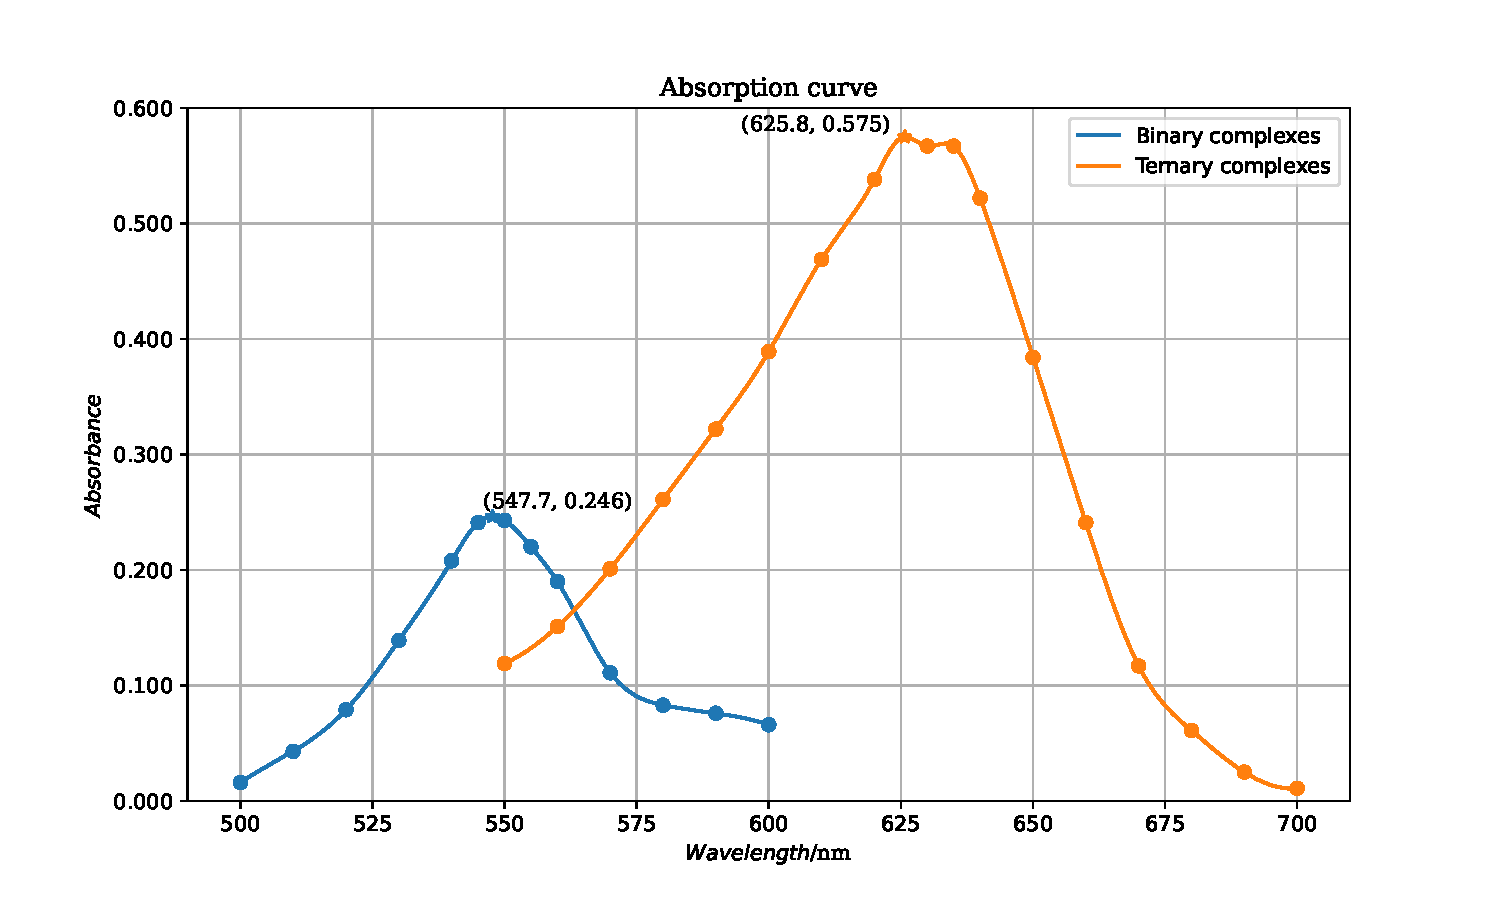
\includegraphics[scale=0.6]{CAS}
	\caption[scale=0.6]{\ce{Al^{3+}}的吸收曲线({\kaishu 横坐标为波长,纵坐标为吸光度,其中蓝色线代表二元络合物,橘色线代表三元络合物})}
 \end{figure}

\end{document}